\documentclass[border=10pt]{standalone}
\usepackage[svgnames]{xcolor}
\usepackage{amsmath}
\usepackage{pgfplots}
\pgfplotsset{compat=newest}
\usepackage[sfdefault]{FiraSans}
\usepackage{FiraMono}
\renewcommand*\familydefault{\sfdefault}
\begin{document}
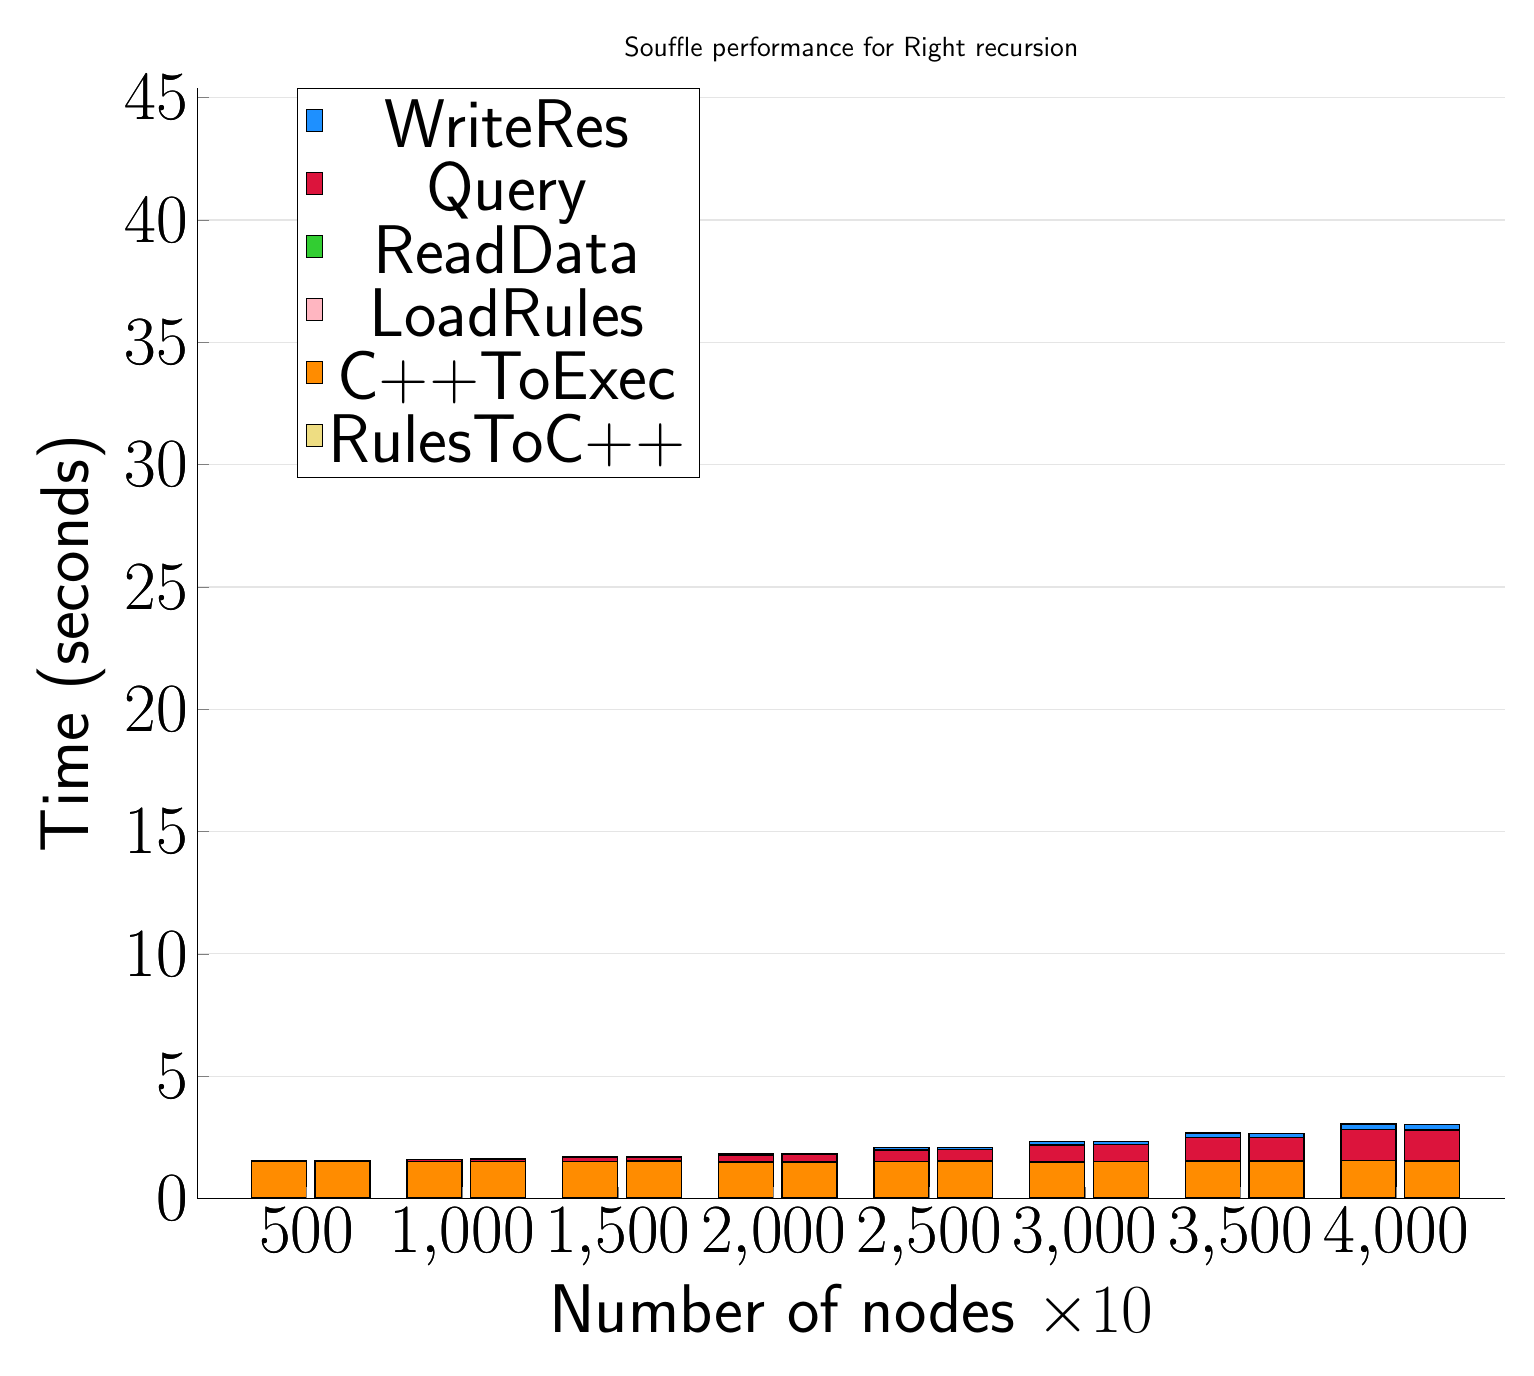
\begin{tikzpicture}
\begin{axis}[
   ybar stacked,
   title={Souffle performance for Right recursion},
   bar shift=-10pt,
   width=1.5\textwidth,
   bar width=0.7cm,
   ymajorgrids, tick align=inside,
   major grid style={draw=gray!20},
   xtick=data,
   ymin=0, ymax=45.40037,
   axis x line*=bottom,
   axis y line*=left,
   enlarge x limits=0.1,
   legend style={
       at={(0.23, 1)},
       anchor=north,
       legend columns=1,
       font=\Huge,
   },
   ylabel={Time (seconds)},
   xlabel={Number of nodes $\times 10$},
   label style={font=\Huge},
   tick label style={font=\Huge},
]
\addlegendimage{fill=DodgerBlue, draw=black, line width=0.2pt}
\addlegendentry{WriteRes}
\addlegendimage{fill=Crimson, draw=black, line width=0.2pt}
\addlegendentry{Query}
\addlegendimage{fill=LimeGreen, draw=black, line width=0.2pt}
\addlegendentry{ReadData}
\addlegendimage{fill=LightPink, draw=black, line width=0.2pt}
\addlegendentry{LoadRules}
\addlegendimage{fill=DarkOrange, draw=black, line width=0.2pt}
\addlegendentry{C++ToExec}
\addlegendimage{fill=LightGoldenrod, draw=black, line width=0.2pt}
\addlegendentry{RulesToC++}
\addplot +[fill=LightGoldenrod, draw=black, line width=0.5pt] coordinates {
    (500, 0.045000004768371585)
    (1000, 0.04100000858306885)
    (1500, 0.04100000858306885)
    (2000, 0.04000003337860107)
    (2500, 0.040999960899353025)
    (3000, 0.039999985694885255)
    (3500, 0.047000002861022946)
    (4000, 0.04400002956390381)
};
\addplot +[fill=DarkOrange, draw=black, line width=0.5pt] coordinates {
    (500, 1.4850000143051147)
    (1000, 1.4719999790191651)
    (1500, 1.4819999933242798)
    (2000, 1.4479999780654906)
    (2500, 1.4790000200271607)
    (3000, 1.4620000123977661)
    (3500, 1.4960000038146972)
    (4000, 1.5089999914169312)
};
\addplot +[fill=LightPink, draw=black, line width=0.5pt] coordinates {
    (500, 0.0)
    (1000, 0.0)
    (1500, 0.0)
    (2000, 1.01583e-05)
    (2500, 0.0)
    (3000, 0.0)
    (3500, 0.0)
    (4000, 0.0)
};
\addplot +[fill=LimeGreen, draw=black, line width=0.5pt] coordinates {
    (500, 0.0011813037)
    (1000, 0.0022576840000000003)
    (1500, 0.003294486)
    (2000, 0.0043747429999999995)
    (2500, 0.005105647)
    (3000, 0.006166652999999999)
    (3500, 0.007239863000000001)
    (4000, 0.008889725)
};
\addplot +[fill=Crimson, draw=black, line width=0.5pt] coordinates {
    (500, 0.01921289)
    (1000, 0.07334286)
    (1500, 0.1612291)
    (2000, 0.2928784)
    (2500, 0.46496139999999997)
    (3000, 0.6846113)
    (3500, 0.951469)
    (4000, 1.254212)
};
\addplot +[fill=DodgerBlue, draw=black, line width=0.5pt] coordinates {
    (500, 0.0045525209999999995)
    (1000, 0.014254779999999998)
    (1500, 0.032977219999999995)
    (2000, 0.056721199999999986)
    (2500, 0.08932446000000001)
    (3000, 0.1281488)
    (3500, 0.1732704)
    (4000, 0.2257253)
};
\end{axis}
\begin{axis}[
   ybar stacked,
   bar shift=13pt,
   width=1.5\textwidth,
   bar width=0.7cm,
   ymajorgrids, tick align=inside,
   major grid style={draw=none},
   xtick=data,
   ymin=0, ymax=45.40037,
   axis x line*=none,
   axis y line*=none,
   enlarge x limits=0.1,
   label style={font=\Huge},
   tick label style={font=\Huge},
]
\addplot +[fill=LightGoldenrod, draw=black, line width=0.5pt] coordinates {
    (500, 0.031000000000000007)
    (1000, 0.030000000000000006)
    (1500, 0.031000000000000007)
    (2000, 0.030000000000000006)
    (2500, 0.030000000000000006)
    (3000, 0.030000000000000006)
    (3500, 0.031000000000000007)
    (4000, 0.03200000000000001)
};
\addplot +[fill=DarkOrange, draw=black, line width=0.5pt] coordinates {
    (500, 1.496)
    (1000, 1.495)
    (1500, 1.4979999999999998)
    (2000, 1.4700000000000002)
    (2500, 1.497)
    (3000, 1.4789999999999999)
    (3500, 1.5050000000000001)
    (4000, 1.504)
};
\addplot +[fill=LightPink, draw=black, line width=0.5pt] coordinates {
    (500, 0.0)
    (1000, 0.0)
    (1500, 0.0)
    (2000, 1.01e-05)
    (2500, 0.0)
    (3000, 0.0)
    (3500, 0.0)
    (4000, 0.0)
};
\addplot +[fill=LimeGreen, draw=black, line width=0.5pt] coordinates {
    (500, 0.0011676)
    (1000, 0.0022436)
    (1500, 0.0032228)
    (2000, 0.0043312)
    (2500, 0.005075500000000001)
    (3000, 0.006135099999999999)
    (3500, 0.007208600000000001)
    (4000, 0.008861399999999998)
};
\addplot +[fill=Crimson, draw=black, line width=0.5pt] coordinates {
    (500, 0.0190286)
    (1000, 0.0731685)
    (1500, 0.160742)
    (2000, 0.2923845)
    (2500, 0.4639656)
    (3000, 0.6832631000000001)
    (3500, 0.9493334000000001)
    (4000, 1.250394)
};
\addplot +[fill=DodgerBlue, draw=black, line width=0.5pt] coordinates {
    (500, 0.004326100000000001)
    (1000, 0.014152799999999998)
    (1500, 0.0322575)
    (2000, 0.056145)
    (2500, 0.08829490000000001)
    (3000, 0.1269263)
    (3500, 0.1719552)
    (4000, 0.2243158)
};
\end{axis}
\end{tikzpicture}

\end{document}
